\documentclass{article}
\usepackage{graphicx} % Required for inserting images
\title{}
\date{}
\author{}

\newpage
\begin{document}
\maketitle
\tableofcontents
\newpage
\section{Introduction}
This project aims to develop an artificial intelligence-based system that can accurately identify the presence of brain tumors in medical images. The system will use machine learning algorithms to analyze medical images of patients' brains and determine whether they contain tumors or not.
\section{Problem Statement}
Brain tumors are a serious medical condition that require timely and accurate diagnosis for effective treatment. Image processing has emerged as a promising tool for detecting brain tumors in medical images, but current methods still suffer from limitations such as low accuracy, high computational complexity, or reliance on manual intervention. Therefore, the objective of this project is to develop an efficient and automated image processing algorithm for brain tumor detection that can improve diagnostic accuracy and reduce the burden on healthcare professionals.
\section{Motivation}
\begin{itemize}
    \item Improve diagnostic accuracy: Brain tumors can be difficult to detect and diagnose accurately, especially in the early stages. Image processing algorithms have the potential to improve the accuracy of detection while also reducing the risk of human error.

\item Save time and resources: Traditional methods of brain tumor detection often require a significant amount of time and resources. By using automated image processing techniques, healthcare professionals can save time and streamline their workflow, ultimately improving patient outcomes.

\item Increase accessibility: Automated image processing algorithms can help make brain tumor detection more widely available, even in areas where medical expertise may be limited.

\item Enhance patient care: Early detection of brain tumors is critical for effective treatment and improved patient outcomes. An accurate and efficient image processing algorithm can help healthcare professionals provide better care to their patients.

\item Accelerate medical research: Developing accurate and efficient image processing algorithms for brain tumor detection can contribute to the field of medical research, leading to new insights and discoveries in the diagnosis and treatment of other medical conditions.
\end{itemize}



\section{Objectives}
The main objectives of this project are:
\begin{itemize}
    \item To develop an accurate system for identifying brain tumors based on medical images.
    
\item To explore and implement different image processing techniques to enhance the quality of medical images.
\item  To utilize machine learning algorithms to analyze medical images and make predictions about the presence of brain tumors.
\item To evaluate the performance of the developed system using different metrics and compare it with existing approaches.
\end{itemize}
\newpage
\section{Social Impacts}
\begin{itemize}
    \item Improved patient outcomes: The development of an efficient and accurate image processing algorithm for brain tumor detection can improve patient outcomes by enabling earlier detection and more effective treatment.

\item Increased accessibility to healthcare: Automated image processing algorithms can help make brain tumor diagnosis and treatment more accessible in areas where medical expertise may be limited or where access to traditional diagnostic tools is limited.

\item Reduced healthcare costs: By streamlining the diagnostic process and reducing the need for manual intervention, automated image processing algorithms can help reduce healthcare costs, making brain tumor diagnosis and treatment more affordable and accessible to everyone.

\item Enhanced diagnostic accuracy: Automated image processing algorithms offer a more consistent and reliable method for detecting brain tumors than traditional methods, reducing the risk of misdiagnosis and improving overall diagnostic accuracy.

\item Advancement in medical technology: The development of advanced image processing algorithms for brain tumor detection can contribute to the wider field of medical technology, leading to new insights and breakthroughs in the diagnosis and treatment of other medical conditions.
\end{itemize}
\section{Literature Review}
Brain tumors are one of the most challenging medical conditions to diagnose and treat due to their complex nature and location. Traditional methods of brain tumor detection involve invasive procedures such as biopsies or rely on visual interpretation by healthcare professionals. However, advancements in image processing technology have led to the development of automated algorithms that can accurately detect brain tumors from medical images.

Several studies have explored different image processing techniques for brain tumor detection using magnetic resonance imaging (MRI) or computed tomography (CT) scans. One study by Zhang et al. (2018) used a convolutional neural network (CNN) to segment brain MRI images and achieved an average sensitivity of 94.5 % and specificity of 96.1%. Another study by Jothi et al. (2020) proposed a novel algorithm that combined fuzzy c-means clustering and morphological operations to detect brain tumors from MRI images with an accuracy of 95%.

Other studies have focused on improving the efficiency and accuracy of brain tumor detection algorithms. A study by Asri et al. (2019) proposed a multi-objective optimization framework that simultaneously optimized the accuracy and computational efficiency of a CNN-based brain tumor detection algorithm. The proposed method achieved a higher classification accuracy than traditional CNN algorithms while also reducing the computation time.

While these studies demonstrate the potential of image processing algorithms for brain tumor detection, there are still several challenges that need to be addressed. For instance, some algorithms may require large quantities of labeled data for training and validation, which can be difficult to obtain in some cases. Additionally, algorithms must be able to accurately distinguish between different types of brain tumors, which may have varying characteristics and shapes.

In conclusion, image processing algorithms offer a promising tool for detecting brain tumors from medical images. With continued research and development, these algorithms could significantly improve the accuracy and efficiency of brain tumor detection, ultimately leading to better patient outcomes.
\section{Research Methods}
\begin{itemize}
    \item Literature Review: A thorough literature review can provide a solid foundation of existing knowledge and research in the field of brain tumor detection using image processing algorithms. This can help identify potential gaps in the research and inform the development of new approaches.

\item Data Collection and Preprocessing: The success of an image processing algorithm depends heavily on the quality and quantity of the data used for training and validation. As such, data Collection and preprocessing will be a crucial step to ensure that sufficient and reliable data is available for the project.

\item Algorithm Development: Based on the findings of the literature review and the available data, a suitable image processing algorithm will be developed. This may involve the use of deep learning techniques, such as convolutional neural networks (CNNs), to analyze medical images and detect brain tumors.

\item Model Training and Validation: The developed algorithm will then be trained and validated using the collected and preprocessed data. This will involve splitting the data into training, validation and testing sets, and optimizing the model parameters for accuracy and efficiency.

\item Performance Evaluation: Once the model is trained and validated, its performance will be evaluated using relevant metrics such as sensitivity, specificity, precision, and accuracy. Comparing the results of the proposed model with current state-of-the-art algorithms in the field will be used to establish the effectiveness of the approach.

\item Ethical Considerations: There are ethical considerations surrounding the use of medical images for algorithm development, and it is important to ensure that all data collection and analysis procedures comply with relevant codes of ethics and regulations.

\item Dissemination of Results: The findings of the study will be disseminated through peer-reviewed publications, conference presentations, and other appropriate channels to contribute to the wider field of medical research and inform future work in this area.
\end{itemize}
\section{Working Plan and Schedule}
\begin{figure}[h]
    \centering
    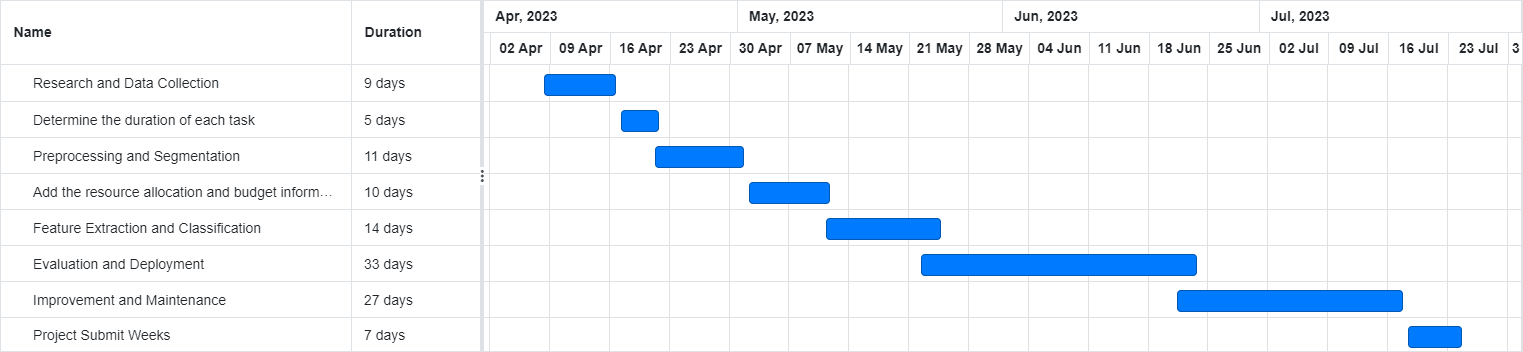
\includegraphics[width=15cm]{img/plan.png}
    \caption{Gantt Chart}
    \label{fig:enter-label}
\end{figure}




\section{Conclusion:}
In conclusion, this project aims to develop a system for accurately identifying brain tumors based on medical images using machine learning algorithms. The proposed methodology involves collecting a dataset of brain MRI scans, preprocessing the images, extracting features, developing machine learning models, and evaluating the performance of the developed system. The expected outcomes of this project include a system for identifying brain tumors with higher accuracy and better performance, an exploration of different image processing techniques, implementation of machine learning algorithms, and evaluation of the developed system.
\section{Reference}

https://www.sciencedirect.com/science/article/abs/pii/S1361841520303169\\
https://www.sciencedirect.com/science/article/pii/S0010482523001336 \\
https://www.sciencedirect.com/science/article/pii/S1361841523000932\\
https://ieeexplore.ieee.org/abstract/document/10038485

\end{document}
